\documentclass[12pt,a4paper]{article}
\usepackage[utf8]{inputenc}
\usepackage{graphicx}
\usepackage{hyperref}
\usepackage{multirow}
\usepackage{booktabs}
\renewcommand{\baselinestretch}{1.2}
\title{Ranking King Saud University Computer Science Curriculum}
\author{Mohand Alrasheed}
\date{2022 / January / 2}

\begin{document}
\pagenumbering{gobble}

\maketitle
\clearpage

\tableofcontents
\clearpage


\section{Introduction}
King Saud University's computer science curriculum has many pros and cons, in this document we outline a criteria for judging courses and ranking the curriculum based on experts' opinions.

\section{Assumptions} 
We make a number of assumptions regarding the evaluation of courses, these guide the evaluation process so they should be read carefully before moving on to results.

\paragraph{Assumptions}
\begin{enumerate}
    \item The course instructor's influence is minimized when ranking courses by imagining all courses being taught by a perfect instructor.
    \item The ranking has been chosen by students mostly on their final semester, which would mean most of them have not studied the last semester and in turn we will not take its courses into consideration in this version.
    \item The ranking has been chosen by students mostly belonging batch 439 and 438, different batches might rank courses differently as course content changes slowly.
    \item Most electives are not taken into consideration, but a small number of popular electives will be considered. 
\end{enumerate}

\section{Criteria}
Courses are judged based on five criteria chosen by the most elite members of 439.

\paragraph{Criteria}
\begin{enumerate}
    \item \textbf{Applications}: This refers to real-world applications of the knowledge gained by studying the course.
    \item \textbf{Relevance}: This refers to the new-ness of the knowledge taught compared to the current (as of this document's date) state of the art.
    \item \textbf{Insight}: This refers to the quality of the knowledge gained with respect to understanding the world and expanding one's horizons.
    \item \textbf{Understanding}: This refers to the proportion of the course's understanding portions over the memorization portions. 
    % \item \textbf{Completeness}: This refers to how connected the course is as a package. A course with randomly assembled useful info will score badly on this category, while a cohesively assembled useless info scores highly.
    \item \textbf{Ease}: This refers to how easy the course was.
\end{enumerate}

\section{Method}
\subsection{Data}
The data is collected and sorted using \emph{Google Forms} in which each reviewer identifies their university batch and sex as well as rate an optional number of courses, i.e. the reviewer can review zero courses, or all courses if they wish. Each reviewer can optionally also provide extra notes alongside any course. 

The number of courses ended up being 42, where we include the core plan as well as popular electives. After filtering courses with too few reviews we end up with a number of reviewers totalled 16 where the minimum number of reviews of any course is 2 and the maximum is 14, the distribution of counts is skewed to the right where the 50th percentile is 11 and the 75th is 13. After collecting the data we end up with (Courses, Criteria) X reviewer matrix.
\subsection{Score calculation}
Due to the low sample size on reviews of some courses we treat the problem as a \emph{Bayesian estimation} problem. In our implementation we possess an idea of the original values we're predicting what we call the \emph{prior}, which in this case will be the arithmetic mean of a criterion on some category\footnote{Categories are divided in this way: Humanities, Mathematics, Chemistry, Islamics, Physics, Computer science}, then we  update our beliefs given new evidence (reviews) by taking a weighted average of the criterion and the prior. \[(r_1 * w_1 + .. + r_n * w_n + c{_m_e_a_n} * w_c)/(\Sigma^n_{i_=_1} w_i + w_c)\]
We experimented with the weight of the category mean \(c_{m_e_a_n}\) and arrived at a weight half as weighty as the weight of the reviews.

After collecting and processing the data we will rank courses using a weighted mean of criteria, we will use three different weights.

\paragraph{Weighing technique}
\begin{enumerate}
    \item \textbf{General}: This weighing takes everything into account fairly, equivalent to a traditional mean. \[Applications\; +\; Relevance\; +\; Insight\; +\; Understanding\; +\; Ease\]
    \item \textbf{Real-world}: This score mainly focuses on real world utility. \[Applications * 1.5\; +\; Relevance\; +\; Insight * 0\; +\; Understanding * 0.2\; +\; Ease * 0.5\]
    \item \textbf{Academic}: This score only focuses on the academic aspect of courses. \[Applications * 0\; +\; Relevance * 0\; +\; Insight * 1.5\; +\; Understanding * 1.5\; +\; Ease * 0\]
\end{enumerate}


\section{Results}
\hskip-1.7cm
\begin{tabular}{lrrrl}
\toprule
{} &  Real-world score &  Academic score &  General score &        categories \\
\midrule
ENGLISH100      &          0.977969 &        0.587055 &       0.749899 &        Humanities \\
ARB100          &          0.644273 &        0.561107 &       0.559423 &        Humanities \\
MATH101         &          0.899391 &        0.883593 &       0.772007 &       Mathematics \\
CHEM101         &          0.520728 &        0.438133 &       0.445344 &         Chemistry \\
STAT101         &          0.927789 &        0.804526 &       0.756429 &       Mathematics \\
TECH101         &          0.765262 &        0.545605 &       0.626730 &        Humanities \\
ENTREPRENEUR101 &          0.601895 &        0.521720 &       0.530546 &        Humanities \\
FAJAB101        &          0.600165 &        0.538924 &       0.546742 &        Humanities \\
NAHAJ101        &          0.638404 &        0.661528 &       0.594242 &        Humanities \\
ENGLISH110      &          0.918583 &        0.582118 &       0.713858 &        Humanities \\
SALAM107        &          0.754027 &        0.638643 &       0.659744 &          Islamics \\
PHYS104         &          0.624921 &        0.534890 &       0.519392 &           Physics \\
MATH106         &          0.794863 &        0.735696 &       0.674323 &       Mathematics \\
CSC111          &          0.984843 &        0.934987 &       0.849246 &  Computer science \\
MATH151         &          0.954951 &        0.868024 &       0.817721 &       Mathematics \\
SALAM108        &          0.634832 &        0.415596 &       0.526326 &          Islamics \\
CSC113          &          0.840633 &        0.775292 &       0.730219 &  Computer science \\
CSC220          &          0.862635 &        0.832111 &       0.739635 &  Computer science \\
MATH244         &          0.831908 &        0.716022 &       0.674008 &       Mathematics \\
CSC212          &          0.943643 &        1.000000 &       0.839300 &  Computer science \\
CSC215          &          0.801212 &        0.781024 &       0.676474 &  Computer science \\
MATH281         &          0.848302 &        0.846393 &       0.748259 &       Mathematics \\
CSC304          &          0.676360 &        0.582436 &       0.612944 &  Computer science \\
CSC380          &          0.795881 &        0.727745 &       0.676944 &  Computer science \\
CSC227          &          0.740514 &        0.637227 &       0.619513 &  Computer science \\
CSC311          &          0.993665 &        0.991418 &       0.866180 &  Computer science \\
CSC339          &          0.671742 &        0.846109 &       0.679513 &  Computer science \\
CSC343          &          0.659292 &        0.501000 &       0.529513 &  Computer science \\
CSC361          &          0.801822 &        0.819164 &       0.703416 &  Computer science \\
CSC329          &          0.971137 &        0.964173 &       0.849513 &  Computer science \\
CSC340          &          0.609492 &        0.737127 &       0.586180 &  Computer science \\
CSC453          &          0.658107 &        0.646309 &       0.582847 &  Computer science \\
CSC496          &          0.898492 &        0.796582 &       0.736309 &  Computer science \\
PHYS103         &          0.611916 &        0.635857 &       0.542905 &           Physics \\
CSC443          &          0.683071 &        0.549409 &       0.578540 &  Computer science \\
CSC462          &          1.000000 &        0.922291 &       0.843796 &  Computer science \\
CSC489          &          0.792190 &        0.732545 &       0.691387 &  Computer science \\
\bottomrule
\end{tabular}

\subsection{Visuals}
We include the most important visualizations done. Which are the general scores ranking and the weighted scores ranking. More visualization and a live demo with interact-able graphs can be found \href{http://courses.hawzen.me}{here}.

\begin{figure}
    \centering
    \hskip-1.7cm \rotatebox[origin=c]{90}{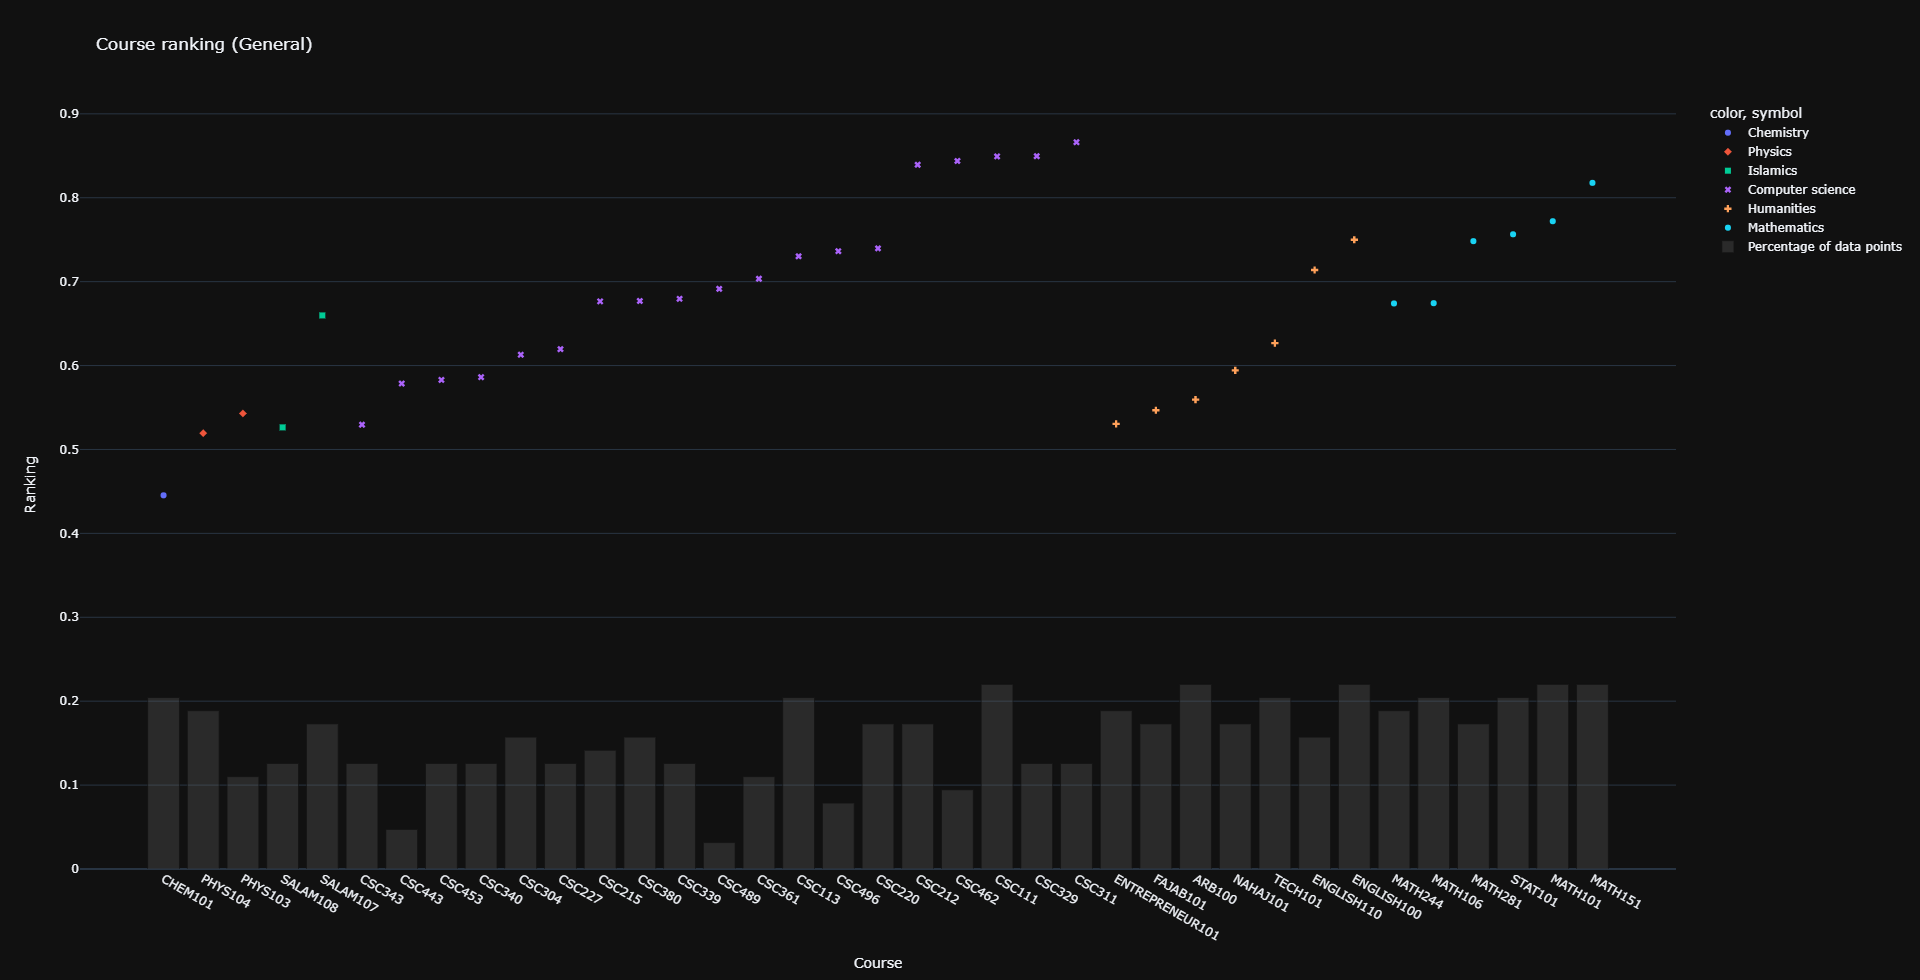
\includegraphics[scale=.3]{normal.png}}
    \caption{Scores based on general ranking}
    \label{fig:my_label}
\end{figure}

\begin{figure}
    \centering
    \rotatebox[origin=c]{90}{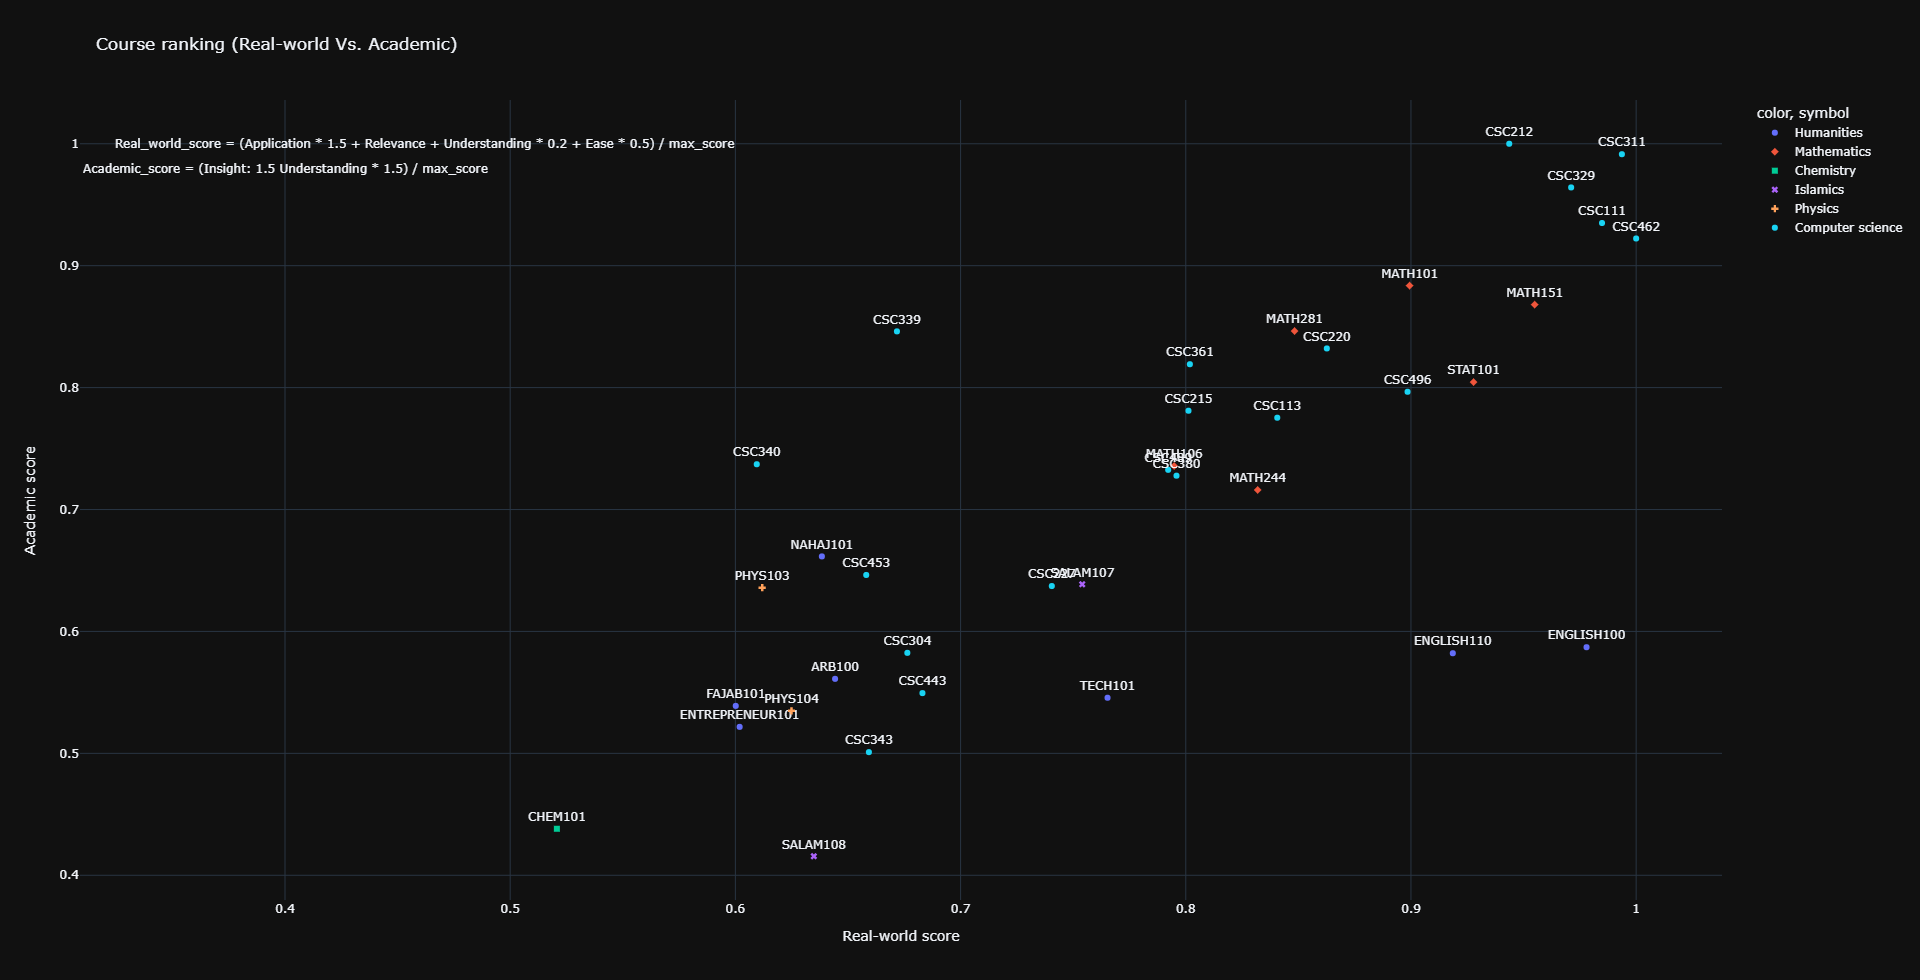
\includegraphics[scale=.3]{weighted.png}}
    \caption{Scores based on Real-world Vs. Academic ranking}
    \label{fig:my_label}
\end{figure}

\clearpage

\subsection{Observations}
Yada yada

\section{Conclusion}
Yada yada

\subsection{Code}
The code can be found at \url{https://github.com/Hawzen/Course-Ranking}
\end{document}
